\subsection{Versuchsaufbau}

\begin{figure}[H]
\begin{center}
  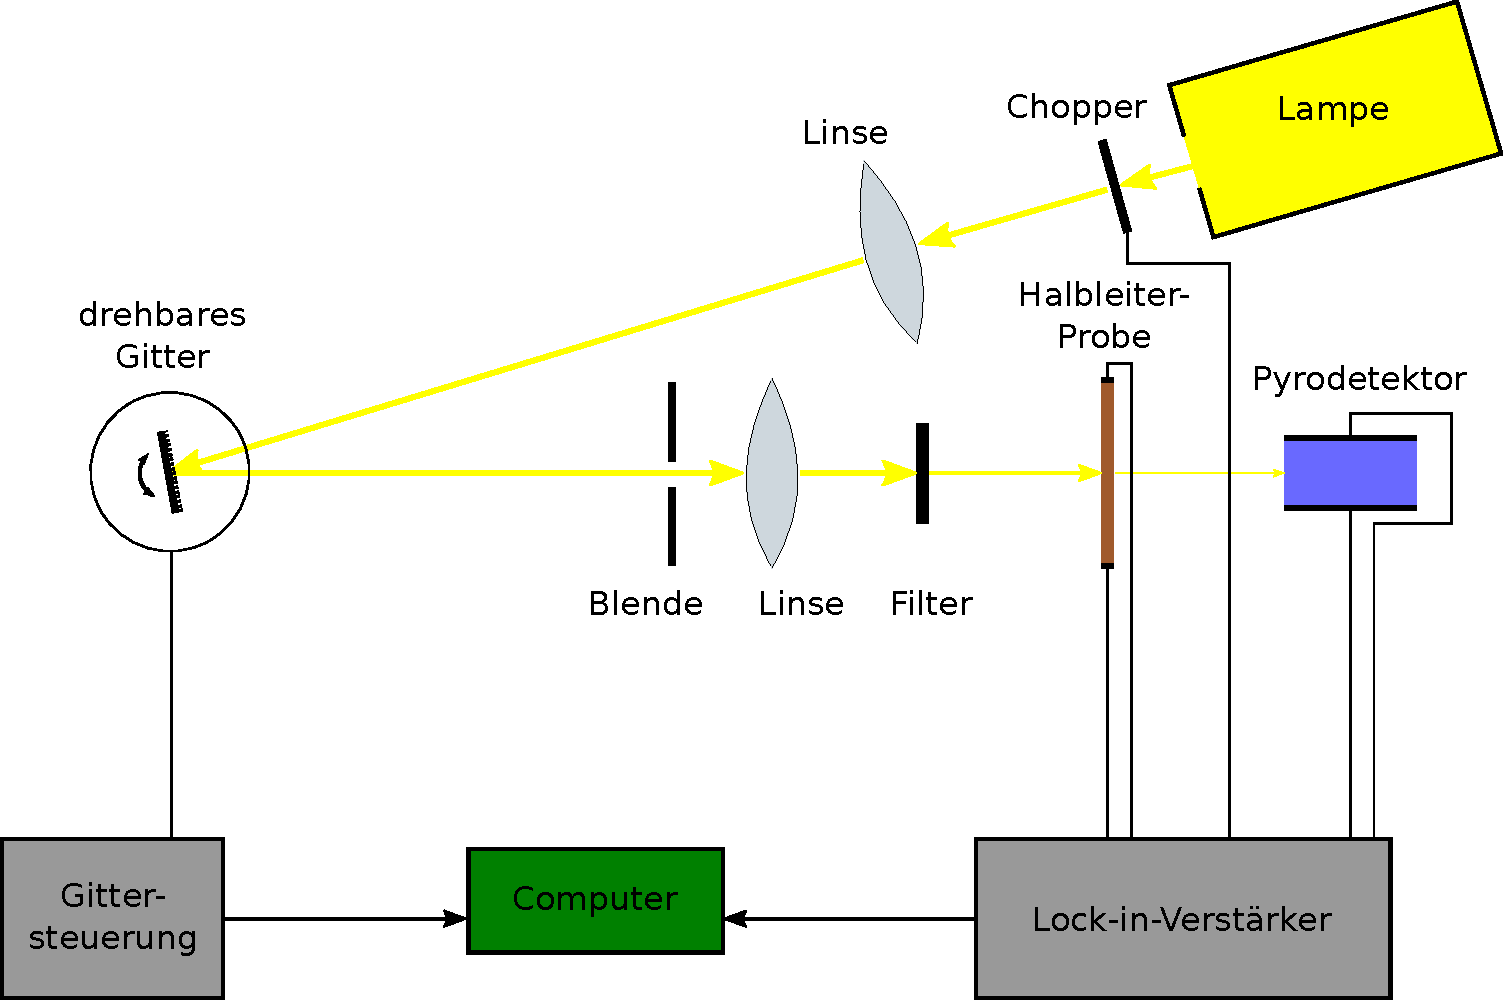
\includegraphics[width=0.9\textwidth]{../img/aufbauBL.pdf}
  \caption{Aufbau zur Messung der Wellenlängenabhängigkeit von
  Absorption und Transmission von Germanium und Silizium.}
  \label{img:aufbauBL}
\end{center}
\end{figure}

\autoref{img:aufbauBL} zeigt den Aufbau, der zur Bestimmung der Bandlücke von Germanium und Silizium
verwendet wird.
Eine Lampe liefert weißes Licht,
das von einem Chopper moduliert und von einer Linse kollimiert wird.
Das Licht wird dann von einem Gitter spektral zerlegt und ein kleiner Teil des Spektrums
gelang durch eine Blende, eine weitere Linse und einen Filter auf die Halbleiterprobe.
Gitter und Filter können ausgetauscht werden.
(Für Silizium wird ein Gitter mit 1200 Linien/mm verwendet und für
Germanium eines mit 600 Linien/mm.
Die beiden Filter lassen nur den langwelligen Bereich des Spektrums passieren.)
Durch den Halbleiter fließt ein Strom, so dass Widerstandsänderungen wegen der
Entstehung von freien Elektronen durch Lichtabsorption detektiert werden können.
Licht, das den Halbleiter transmittiert,
gelangt auf einen Pyrodetektor, der über eine Änderung seiner Dielektrizitätskonstante die
auftretenden Temperaturschwankungen in ein Spannungssignal wandelt.
Dieses Spannungssignal gelangt ebenfalls in den Lock-in-Verstärker.
Um gezielt die Signale von Halbleiter und Pyrodetektor verstärken zu können,
erhält der Verstärker außerdem Information über Frequenz und Phase des modulierten Lichtsignals von Chopper.\\
Das optische Gitter wird über einen Motor angesteuert und die aktuelle Winkelstellung
zusammen mit dem Ausgangssignal
des Verstärkers an einen Computer gesendet.


